
\chapter{Einführung}
\label{cha:einf}

Für die Entwicklung eines Multicast Test Tools mit unten stehenden Fähigkeiten
ist ein Zeitraum vom 21. Oktober 2010 bis 06. Mai 2011 veranschlagt worden. Dieser Zeitraum beinhaltet sowohl die eigentliche
Entwicklungszeit, als auch Planungs- und Konzeptions- und Testphasen.\\
\\
Eingesetzt werden soll das Multicast Test Tool für die Konfigurationsverifikation
eines Local-Area-Networks. Diese umfasst sowohl die Hardware- als auch die
Softwarekomponenten. Dadurch sollen Synchronität und Gleichlauf des gesamten
Netzwerkes überprüft und gegebenenfalls verbessert werden. Das Tool soll es ebenfalls ermöglichen, die Multicast-Fähigkeiten eines
Netzwerkes zu erfassen und zu validieren. Die Darstellung der Ergebnisse soll
möglichst übersichtlich und schnell erfassbar sein.\\
\\

Um diese Anforderungen zu erfüllen, wurden folgende Ziele definiert:\\
Es muss möglich sein mehrere (mindestens 30) Multicast Streams simultan
innerhalb eines Local-Area-Netzwerkes zu senden und zu empfangen. Zusätzlich
werden Statisiken für die Überprüfung benötigt. Hierfür werden Traversierungszeit,
Empfangsintervalle, sowie Anzahl der verlorengegangenen Pakete ermittelt und dem
Nutzer sichtbar gemacht.\\
\\
Um die Testbarkeit von verschiedenen Knotenpunkten innerhalb des Netzes zu
ermöglichen muss eine möglichst plattformunabhängige Lösung entwickelt werden. Hauptsächlich müssen Windows- 
sowie Linuxsysteme unterstüzt werden. \\
\\
Für eine möglichst übersichtliche und komfortable Benutzeroberfläche werden
Empfänger- und Senderprogramm zusammengefasst. 

\chapter{Projektorganisation}
\label{cha:proo}

\section{Beteiligte}

\begin{table}[htdp]
\caption{Beteiligte und Rollenverteilung}
\label{tab:beteiligte}
\begin{center}
\begin{tabular}{|c|c|c|}
\hline
\textbf{Name} & \textbf{Rolle} & \textbf{Grad der Befugnis} \\
\hline
Hildenbrand, David (DH) & Projekt Manager & 3 \\
\hline
Jedele, Jeffrey (JJ) & Leitender Ingenieur & 1 \\
\hline
Safarpour, Ramin (RS) & Systemtest & 1 \\
\hline
Schoknecht, Tobias (TSC) & Dokumentation & 1 \\
\hline
Stöckel, Tobias (TST) & Produkt Manager & 2 \\
\hline
Weitz, Konstantin (KW) & Leitender Ingenieur & 1  \\
\hline
\end{tabular}
\end{center}
\label{default}
\end{table}

\section{Stakeholder}

\begin{table}[htdp]
\caption{Stakeholder}
\label{tab:stakeholder}
\begin{center}
\begin{tabular}{|c|c|c|}
\hline
\textbf{Name} & \textbf{Kurzbeschreibung}\\
\hline
Andreas Stuckert & Mitarbeiter Fa. Net-Tools \\
\hline
Markus Rentschler & Mitarbeiter Fa. Net-Tools \\
\hline
Fa. Net-Tools & Auftraggebende Firma \\
\hline
Fa. SPAM & Entwickelnde Firma \\
\hline
Teammitglieder & siehe Tabelle \ref{tab:beteiligte} \\
\hline
\end{tabular}
\end{center}
\label{default}
\end{table}

\chapter{Entwicklungsmodell}
\label{cha:entw}

\paragraph {Entwicklungsteam}
Innerhalb des Projektteams wird nach dem Wasserfallmodell entwickelt. Die
Begründung hierfür ist, dass für ein Projekt mit diesem Umfang das Verwenden des
V-Modells schlichtweg unverhältnismäßig ist. Bei kleineren Projekten ist es
unnötig einen solchen Aufwand besonders im Bezug auf die sehr exakte
Dokumentation zu betreiben. Das Vorgehen nach dem im folgenden
beschriebenen Wasserfallmodell ist für das Projekt angemessen.\\
\\
Das Wasserfallmodell zeichnet sich dadurch aus, dass die einzelnen Phasen
sequentiell durchlaufen werden, es ist allerdings möglich in eine frühere Phase
zurückzukehren, sollte dies notwendig sein. Zum Abschluss einer Phase müssen
Gates passiert werden, die Ergebnisse werden in Ergebnisdokumenten
festgehalten. Zu Beginn des Projektes müssen CRS und SRS als wichtigste Dokumente erstellt
werden.

\paragraph{Extern}
Nach außen hin kann das Entwicklungsmodell als inkrementell angesehen werden. Da
beide Seiten an einer längerfristigen Geschäftsbeziehung interessiert sind und
nicht alle wünschenswerten Features Teil des Tools werden können, ist es geplant für die
Firma Net-Tools in den folgenden Jahren neue Versionen zu entwickeln. Eventuelle
Features und nicht dringend notwendige, aber von Kundenseite gewünschte
Funktionen können so später verfügbar gemacht werden. Außerdem ermöglicht
dieses Vorgehen die Software auch auf zukünftige Wünsche und Anforderungen
anzupassen.
%Innen: Waterfall Modell(Phasen-Modell)
%Nach außen: Iterativ -> Versionen

\chapter{Risikoanalyse und FMEA}
\label{cha:risi}

\section{Produktrisiken}
\label{sec:prorisk}

\paragraph{/R0100/}Hardwareausfälle \\
\texttt{Beschreibung:} Da Multicasting von vielen Netzwerkkomponenten nicht richtig unterstützt wird, könnte der Einsatz des Tools zu Hardwareausfällen führen.\\
\texttt{Wahrscheinlichkeit:} mittel\\
\texttt{Entdeckbarkeit:} hoch\\
\texttt{Schaden:} mittel\\
\texttt{Vermeidung:} Nicht möglich.\\
\texttt{Reaktion:} Austausch der Hardware.\\

\paragraph{/R0200/}Netzwerküberlastung\\
\texttt{Beschreibung:} Die Verwendung des Tools von ungeschulten Benutzern kann, wegen der Beschaffenheit von Multicast Protokollen, zu einer Netzüberlastung führen. \\
\texttt{Wahrscheinlichkeit:} mittel\\
\texttt{Entdeckbarkeit:} hoch\\
\texttt{Schaden:} gering\\
\texttt{Vermeidung:} Gute Dokumentation und Schulung der Benutzer.\\
\texttt{Reaktion:} Abschalten des Tools.\\

\section{Marktrisiken}
\label{sec:marketrisk}

\paragraph{/R1000/}Mitbewerber\\ 
\texttt{Beschreibung:} Der Fakt dass es vier direkte Mitbewerber gibt, die ein
Produkt für die exakt gleiche Zielgruppe entwickeln, könnte zum Untergang des
Produktes im Markt führen. \\ \texttt{Wahrscheinlichkeit:} mittel\\ \texttt{Entdeckbarkeit:} gering\\
\texttt{Schaden:} hoch\\
\texttt{Vermeidung:} Hohe Qualität des Tools.\\
\texttt{Reaktion:} Anpassen des Tools für Nischenbereiche.\\

\paragraph{/R1100/}Fähigkeiten der Entwickler\\
\texttt{Beschreibung:} Da das Team noch sehr wenig Praktische Erfahrung mit
Softwareprojekten sammeln konnte, sind starke Abweichungen bei dem geplanten Zeitaufwand bis zur Fertigstellung, den benötigten Resourcen und der Qualität des Endproduktes sehr wahrscheinlich. \\ 
\texttt{Wahrscheinlichkeit:} mittel\\
\texttt{Entdeckbarkeit:} mittel\\
\texttt{Schaden:} mittel\\
\texttt{Vermeidung:} Experten um Rat fragen, erhöhte Sorgfalt bei der Planung.\\
\texttt{Reaktion:} Reevaluierung der Schätzungen.\\
 
 \section{Entwicklungs Risiken}
 \label{sec:devrisk}

 \paragraph{/R2000/}Echtzeitfähigkeit\\
 \texttt{Beschreibung:} Java könnte durch seine Hardwareabstraktion und
 Speicherbereinigung die hohen Anforderungen an Echtzeitfähigkeit verfehlen. \\ \texttt{Wahrscheinlichkeit:} gering\\
 \texttt{Entdeckbarkeit:} hoch\\
 \texttt{Schaden:} mittel\\
 \texttt{Vermeidung:} Testcases entwickeln. \\
 \texttt{Reaktion:} Wechsel der Programmiersprache.\\

 \paragraph{/R2100/}Plattformabstraktion\\
 \texttt{Beschreibung:} Durch Javas hohe Plattformabstraktion könnten Zugriffe
 auf niedriger Ebene, um zum Beispiel die Netzwerkkarte anzusprechen, nicht
 erlaubt sein. \\ \texttt{Wahrscheinlichkeit:} gering\\ \texttt{Entdeckbarkeit:} hoch\\
 \texttt{Schaden:} mittel\\
 \texttt{Vermeidung:} Testcases entwickeln.\\
 \texttt{Reaktion:} Schreiben der benötigten Komponenten in einer anderen Sprache.\\


%\section{FMEA}
%\label{sec:fmea}
\begin{table}
\caption{FMEA}
\begin{tabular}{|m{2cm}|m{2cm}|m{2cm}|m{2cm}|m{2cm}|m{0.3cm}|m{0.3cm}|m{0.3cm}|m{1cm}|}
\hline
\multicolumn{4}{|c|}{Multicast Test Tool} & 
\multicolumn{5}{c|}{Derzeitiger Zustand} \\
%\multicolumn{2}{|c|}{Veränderungen}       &
%\multicolumn{5}{|c|}{Geänderter Zustand}
\hline
Merkmal & potentielle Fehler & potentielle Folgen & potentielle Ursachen & Verhütung und Prüfung &
\begin{sideways}Auftreten\end{sideways} & \begin{sideways}Bedeutung\end{sideways} & \begin{sideways}Entdeckung\end{sideways} & \begin{sideways}Risiko\end{sideways} \\
\hline
\multirow{8}{1.9cm}{Multicast, > 30 Pakete/s, GUI und CLI, Hirschmann Kompabilität, } &
\multirow{4}{1.9cm}{Nicht ausrechende Fähigkeiten der Entwickler} & 
\multirow{2}{1.9cm}{Verzögerung des Projekts} &
Schlechtes Design & Viele Resourcen in SAS & 3 & 7 & 6 & 126 \\
\cline{4-9}
& & & Aufwands Fehleinschätzung & Große Zeit Puffer & 5 & 5 & 2 & 50 \\
\cline{3-9}
& & \multirow{2}{1.9cm}{Mangelnde Qualität} &
Logische Programmierfehler & Viele Testcases & 7 & 7 & 2 & 98 \\ 
\cline{4-9}
& & & Schlechte Erweiterbarkeit & Viele Resourcen in SAS & 3 & 4 & 5 & 60 \\
\cline{2-9}

& \multirow{4}{1.9cm}{Environment Probleme} &
\multirow{2}{1.9cm}{Java kann nicht verwendet werden} &
Nicht genügend Datenströme & Multicast Tests & 3 & 7 & 6 & 126 \\
\cline{4-9}
& & & Garbage Collector ist zu unberechenbar & Garbage Collector Tests & 5 & 7 & 6 & 210 \\
\cline{3-9}
& & \multirow{2}{1.9cm}{Multicast Library kann nicht verwendet werden} &
Nicht alle Features werden Unterstützt & Lesen der API Spezifikation & 5 & 7 & 2 & 70 \\ 
\cline{4-9}
& & & Library ist zu langsam & Library Tests & 3 & 4 & 5 & 60 \\ 
\hline
\end{tabular}
\end{table}

\chapter{Anforderungen an Hard- und Software}
\label{cha:anfo}

\section{Hardware}
\label{sec:hard}

Jeder Beteiligte benötigt ein Notebook mit 100mbit Ethernet Netzwerkkarte zum
Entwickeln und zum Testen. Diese sind bereits vorhanden und müssen nicht
zusätzlich angeschafft werden.\\ Zusätzlich wird ein Local-Area-Netzwerk
benötigt. Hierzu sind zwei Ethernet-Router mit mindestens 100mbit notwendig. Auch diese Geräte sind bereits
vorhanden.\\
Zum Testen in einem größeren LAN steht die Infrastruktur der DHBW-Stuttgart zur
Verfügung.

\section{Software}
\label{sec:soft}

Sämtliche benötigte Software ist entweder frei nutzbar oder es liegen die
entsprechenden Lizenzen bereits vor. Es muss keine zusätzliche Software
eingekauft werden.

\begin{table}[htdp]
\caption{Verwendete Software}
\label{tab:software}
\begin{center}
\begin{tabular}{|p{4.5cm}|p{5.5cm}|p{5cm}|}
\hline
\textbf{Name} & \textbf{Kurzbeschreibung} & \textbf{Anwendungsgebiet}\\
\hline
Eclipse Java & Entwicklungsumgebung für Java & Entwicklung \\
\hline
MS Project & Unterstützende Projektverwaltungssoftware & Projektverwaltung  \\
\hline
Redmine & Online Projektverwaltungssoftware & Projektverwaltung\\
\hline
Selenic Mercurial & Repository & Entwicklung, Dokumentenerstellung\\
\hline
Visual Paradigm & UML Entwurfsprogramm & Dokumentenerstellung, Planung\\
\hline
TeXlipse Eclipse Plugin & Entwicklungstool für LaTeX Dokumente &
Dokumentenerstellung, Dokumentation\\
\hline
Mercurial Eclipse Plugin & Mercurial Support für Eclipse & Entwicklung, 
Dokumentenerstellung\\
\hline
OmniGraffle & Diagrammerstellungssoftware für Mac OSX & Dokumentenerstellung\\
\hline
OmniPlan & Projektverwaltungssoftware zur Gantt-Diagrammerstellung für Mac OSX & Projektverwaltung, Dokumentenerstellung\\
\hline
Apache Maven & Java Build-Management-Tool & Entwicklung\\
\hline
Apache Continuum & Apache Maven Weboberfläche bzw. Build-Management & Entwicklung\\
\hline
Apache Archiva & Repository für Maven und Continuum & Entwicklung\\
\hline
\end{tabular}
\end{center}
\label{default}
\end{table}

% owner: jeffrey

\chapter{Projektzeitplan und Zuständigkeiten}
\label{cha:proz}

\begin{longtable}[h]{| l | l | l | p{7.5cm} |}
\hline
\bf{Id} & \bf{Fertigstellung} & \bf{Verantwortung} & \bf{Beschreibung}\\
\hline\hline
\endfirsthead
\multicolumn{4}{|c|}{\bf{Milestone 1: Anforderungsanalyse und -definition}}\\
\hline
AP1.1 & 21sep2010 & TST & Analyse der vorhandenen Software\\
AP1.2 & 23sep2010 & TST & Anforderungsbesprechung mit Kunde\\
AP1.3 & 05okt2010 & TST & Fertigstellung CRS, Präsentation\\
AP1.4 & 07okt2010 & TST,DH & Präsenation CRS beim Kunden\\
GATE1.5 & 08okt2010 & - & Abnahme CRS durch Kunden\\
AP1.6 & 01nov2010 & DH,JJ,KW,TST & Fertigsgtellung SRS\\
AP1.7 & 15nov2010 & TST,JJ & Präsentation SRS\\
GATE1.8 & 16nov2010 & - & Abnahme SRS durch Kunden\\
\hline
\multicolumn{4}{|c|}{\bf{Milestone 2: Systementwurf}}\\
\hline
AP2.1 & 11okt2010 & JJ & Festlegung zu verwendender Komponenten und
Technologien\\
AP2.2 & 20okt2010 & JJ,KW & Entwurf der Systemarchitektur\\
AP2.3 & 25okt2010 & JJ,KW & Definition von Systemkomponenten\\
AP2.4 & 12nov2010 & DH & Zuweisung Arbeitspakete an Bearbeiter\\
AP2.5 & 12nov2010 & KW & Fertigstellung SAS\\
GATE2.6 & 12nov2010 & DH,TST,JJ,KW & Abnahme von SAS durch Projektleiter,
Produktmanager sowie den leitenden Ingenieuren\\
\hline
\multicolumn{4}{|c|}{\bf{Milestone 3: Implementierung}}\\
\hline
AP3.1 & 20nov2010 & JJ & Anpassung der Arbeitspakete an Entwicklungsmodell sowie
unterstützendes Tooling\\
AP3.2 & 15feb2011 & separat & Fertigstellung: Implementierung der
Systemkomponenten\\
AP3.3 & 28feb2011 & RS & Fertigstellung: Dokumentation der Systemkomponenten\\
GATE3.4 & 02mar2011 & - & Abnahme der Module durch Projektleiter,
Produktmanager sowie den leitenden Ingenieuren\\
\hline
\multicolumn{4}{|c|}{\bf{Milestone 4: Systemintegration und Test}}\\
\hline
AP3.4 & 28feb2011 & JJ,KW &Zusammenführung des Gesamtsystems\\
AP4.1 & 18mar2011 & TSC & Abschluss aller Komponententests und Testberichte\\
AP4.2 & 25mar2011 & TSC,JJ,KW & Auswertung der Testberichte\\
AP4.3 & 17apr2011 & JJ,KW & Verfeingerung, Bugfixing\\
AP4.4 & 28apr2011 & TSC & finaler Testbericht\\
GATE4.5 & 30apr2011 & JJ,KW & Abnahme Gesamtsystem inkl. Testbericht durch
leitende Ingenieure\\
\hline
\multicolumn{4}{|c|}{\bf{Milestone 5: Übergabe und Einführung}}\\
\hline
AP5.1 & 01may2011 & TSC & Optimierung und Fertigstellung der
Systemdokumentation\\
AP5.2 & 03may2011 & JJ & Deploymentmethode wählen und realisieren\\
AP5.3 & 03may2011 & TST & Präsentation des Endproduktes fertigstellen\\
AP5.4 & 06may2011 & TST & Produktpräsentation und Übergabe\\
GATE5.5 & 06may2011 & - & Produktabnahme durch Kunde\\
AP5.6 & 15may2011 & TST & Schulungswünsche mit Kunde klären\\
AP5.7 & 31may2011 & DH & Arbeitsaufwände in Rechnung stellen\\
\hline
\caption{Milestone-Liste}
\end{longtable}

\clearpage

\begin{landscape}
\begin{figure}
\centering
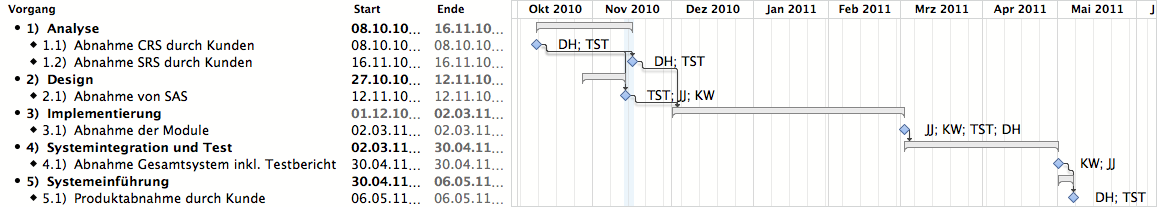
\includegraphics[width=22cm]{images/Projekt-Gantt.png}
\caption{Gantt-Diagramm}\label{fig:gantt}
\end{figure}
\end{landscape}

\chapter{Modulzeitplan und Zuständigkeiten}
\label{cha:modu}
Während der Designphase wurden die folgenden Module identifiziert:

\begin{table}[h]
\caption{Module und Zuständigkeiten}
\label{tab:modz}
\begin{center}
\begin{tabular}{|l|c|p{8cm}|}
\hline
\textbf{Modulname} & \textbf{Verantwortung} & \textbf{Beschreibung}\\
\hline
GUI-Design & TST & Design der grefischen Benutzer Oberfläche\\
\hline
GUI-Logik & TSC & Logik, die hinter der Gui steckt. Konfiguration, Aktualisierung, Listener.\\
\hline
Controller/Profile & DH & Entwicklung des Controllers inklusive der Profil-Verwaltung, Speicherung und dem Laden.\\
\hline
CLI/Logger & RS & Entwicklung der Konsolenschnitstelle inklusive des Loggers.\\
\hline
Sender/Receiver & JJ & Multicast Sende/Empfangsmöglichkeit inklusive der Verwaltung und der Logik.\\
\hline
Paket & KW & Paketdesign und Implementierung.\\
\hline
Language & KW & Entwurf und Verwaltung der Spracheinstellungen.\\
\hline
Installer & KW & Einfache Installation auf Windows und unter Linux Debian.\\
\hline
\end{tabular}
\end{center}
\label{default}
\end{table}

\clearpage

\begin{landscape}

Die Startzeiten sind je nach Fertigstellung der Arbeitspakete noch variabel. Die Endzeiten sind jedoch fix und müssen unbedingt eingehalten werden.
\begin{table}[h]
\caption{Modulzeitplan}
\label{tab:modz}
\begin{center}
\begin{tabular}{|l|c|c|c|c|c|c|}
\hline
\textbf{Modulname} & \textbf{Start} & \textbf{Ende} & \textbf{Zeit Design} & \textbf{Zeit Impl.} & \textbf{Zeit Integration und Test} & \textbf{Zeit Ges.}\\
\hline
GUI-Design & 01dez2010 & 20jan2011 & 2 MT & 8 MT & 5 MT & 15 MT\\
\hline
GUI-Logik &  01dez2010 & 30jan2011 & 3 MT & 8 MT & 6 MT & 17 MT\\
\hline
Controller/Profile &  01dez2010 & 20jan2011 & 3 MT & 8 MT & 5 MT & 16 MT\\
\hline
CLI/Logger &  01dez2010 & 30jan2011 & 2 MT & 8 MT & 3 MT & 13 MT\\
\hline
Sender/Receiver & 01dez2010 & 10jan2011 & 6 MT & 9 MT & 7 MT & 22 MT\\
\hline
Paket & 01dez2010 & 01jan2011 & 2.5 MT & 4 MT & 6 MT & 12.5 MT\\
\hline
Language &  01jan2010 & 20jan2011 & 0.5 MT & 4 MT & 4 MT & 8.5 MT\\
\hline
Installer &  28jan2010 & 10feb2011 & 1 MT & 4 MT & 2 MT & 7 MT\\
\hline
\textbf{Gesamt} & \textbf{01dez2010} & \textbf{10feb2011} & \textbf{20 MT} & \textbf{53 MT} & \textbf{38 MT} & \textbf{111 MT}\\
\hline
\end{tabular}
\end{center}
\label{default}
\end{table}
\end{landscape}

\clearpage

\begin{landscape}
\begin{figure}
\centering
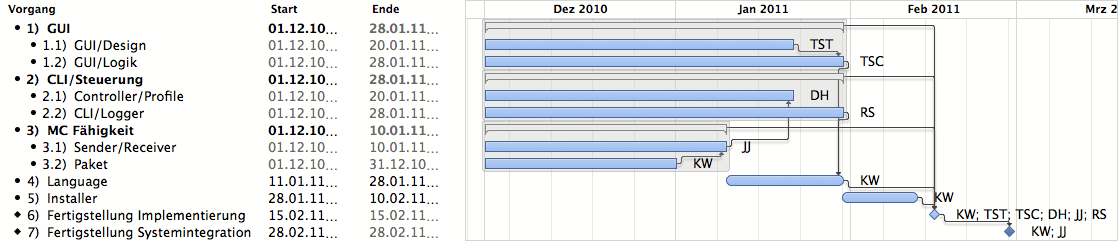
\includegraphics[width=22cm]{images/Modul-Gantt.png}
\caption{Gantt-Diagramm}\label{fig:gantt}
\end{figure}
\end{landscape}

\begin{figure}[h]
\centering
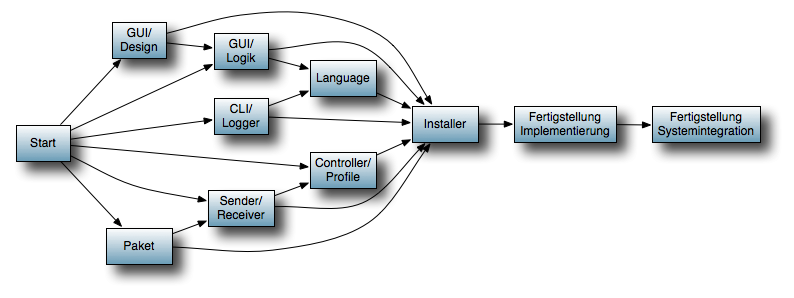
\includegraphics[width=16.5cm]{images/Modul-Netz.png}
\caption{Modul-Implementierung Netzdiagramm}\label{fig:modulnetz}
\end{figure}

Die beiden GUI Module besitzen eine Ende-zu-Ende Abhängigkeit.\\
Sender/Receiver und Controller/Profile besitzen eine Ende-zu-Ende Abhängigkeit und müssen viel wärend der Entwicklung zusammenarbeiten.\\
Sender/Receiver und Paket besitzen eine Ende-zu-Ende Abhängigkeit und müssen sich wärend der Entwicklung abstimmen.\\
GUI-Design und Language besitzen eine Ende-zu-Ende Abhängigkeit.\\
CLI/Logger und Language besitzen eine Ende-zu-Ende Abhängigkeit.\\
Installer besitzt eine Ende-zu-Ende Abhängigkeit zu allen anderen Modulen.\\


\chapter{Überwachung und Berichterstattung}
\label{cha:über}

\paragraph{Meetings}
Meetings finden im wöchentlichen Rhythmus statt. Der exakte nächste Termin wird
jeweils eine Woche im Voraus abgestimmt. Falls der Termin nicht wahrgenommen
werden kann, muss dies unverzüglich dem Projektleiter mitgeteilt werden.
\paragraph{Protokolle}
Zu jedem Treffen wird ein Protokoll angelegt, in dem die anwesenden Teilnehmer,
getroffenen Entscheidungen sowie Arbeitszuweisungen protokolliert werden.
\paragraph{Berichterstattung}
Berichterstattung erfolgt mündlich bei den wöchentlichen Meetings. Kann ein
Termin nicht wahrgenommen werden, so muss der Bericht schriftlich oder per Email
bei dem Projektleiter abgegeben werden. Im Falle von schwerwiegenden Problemen, die den
weiteren Fortschritt des Projekts gefährden könnten, ist sofort der
Projektleiter zu verständigen. Er informiert darauf hin die entsprechenden Mitarbeiter.
\paragraph{Unterstützende Software}
Projektunterstützend wird das online Projektverwaltungstool "`Redmine"'
verwendet. Hier werden alle zugewiesenen Tasks verwaltet. Der Status der
Bearbeitung ist von den Bearbeitern mindestens wöchentlich zu aktualisieren.
Neue zugewiesene Aufgaben müssen beachtet werden.


